% ======================================================================
% DRAFT (2026-10-12): new section on escape dynamics. To be \input after Sec. "Shapes" once the steady-state tests
% (steadyE, hazard) and the circle lambda scan are in. Numbers: RESEARCH.md entries 2026-10-11/12.
% ======================================================================
\section{How a wall defect leaves: escape dynamics}\label{sec:escape}
The shape sweep (Sec.~\ref{sec:shapes}) showed that elongated cavities lose wall defects by single escapes. Here we follow those escapes in time. We keep only
\emph{depleting} escapes: a resident wall $+\half$ (in the 4-cell wall band for at least 40\,t.u.) leaves a layer that already holds at most $2k-2$ defects, no other
defect takes its place, and the vacancy persists for 10--50\,t.u. These are the events that empty the layer. They are 11--12\% of all escapes; the rest are visitors
leaving a crowded layer or swaps. Data: the shape sweep (defects every 2\,t.u.; $\approx1640$ depleting escapes) for tilt and elastic energy, and 36 runs with flow and defects
every 2\,t.u. (area 2500, $k=6$, aspect 1--2; 411 depleting escapes) for everything involving the flow. All curves are aligned on the departure frame (escaper deeper than 6 cells within 20\,t.u.).

\paragraph{Elasticity does not let go (Fig.~\ref{fig:etsg}).} We computed the Frank energy of the measured defect configurations (point-defect model, anisotropic, cores relaxed)
with the escaper displaced along the inward normal.
\begin{itemize}
  \item The restoring force on the escaper stays at $F_0\approx-11$ to $-14\,\kT$/cell (negative pulls towards the wall) up to and through departure, at every aspect and size. It is
        indistinguishable from residents' and even grows slightly as the defect moves out.
  \item The cost of moving 6 cells in drops only in the last $\approx10$\,t.u., by 8--12\,$\kT$: that is the defect leaving, not a precursor.
  \item In elongated cavities (aspect $\ge1.4$) escape sites are elastically cheaper than residents' by 4--5\,$\kT$ from at least 40\,t.u. before (about 10\,$\kT$ at aspect 2.5; none in circles
        or at 1.2). This is a standing property of the site, about 10--15\% of the barrier, not a trigger.
\end{itemize}
So the escaper leaves against an intact elastic barrier.

\begin{figure}[H]\centering
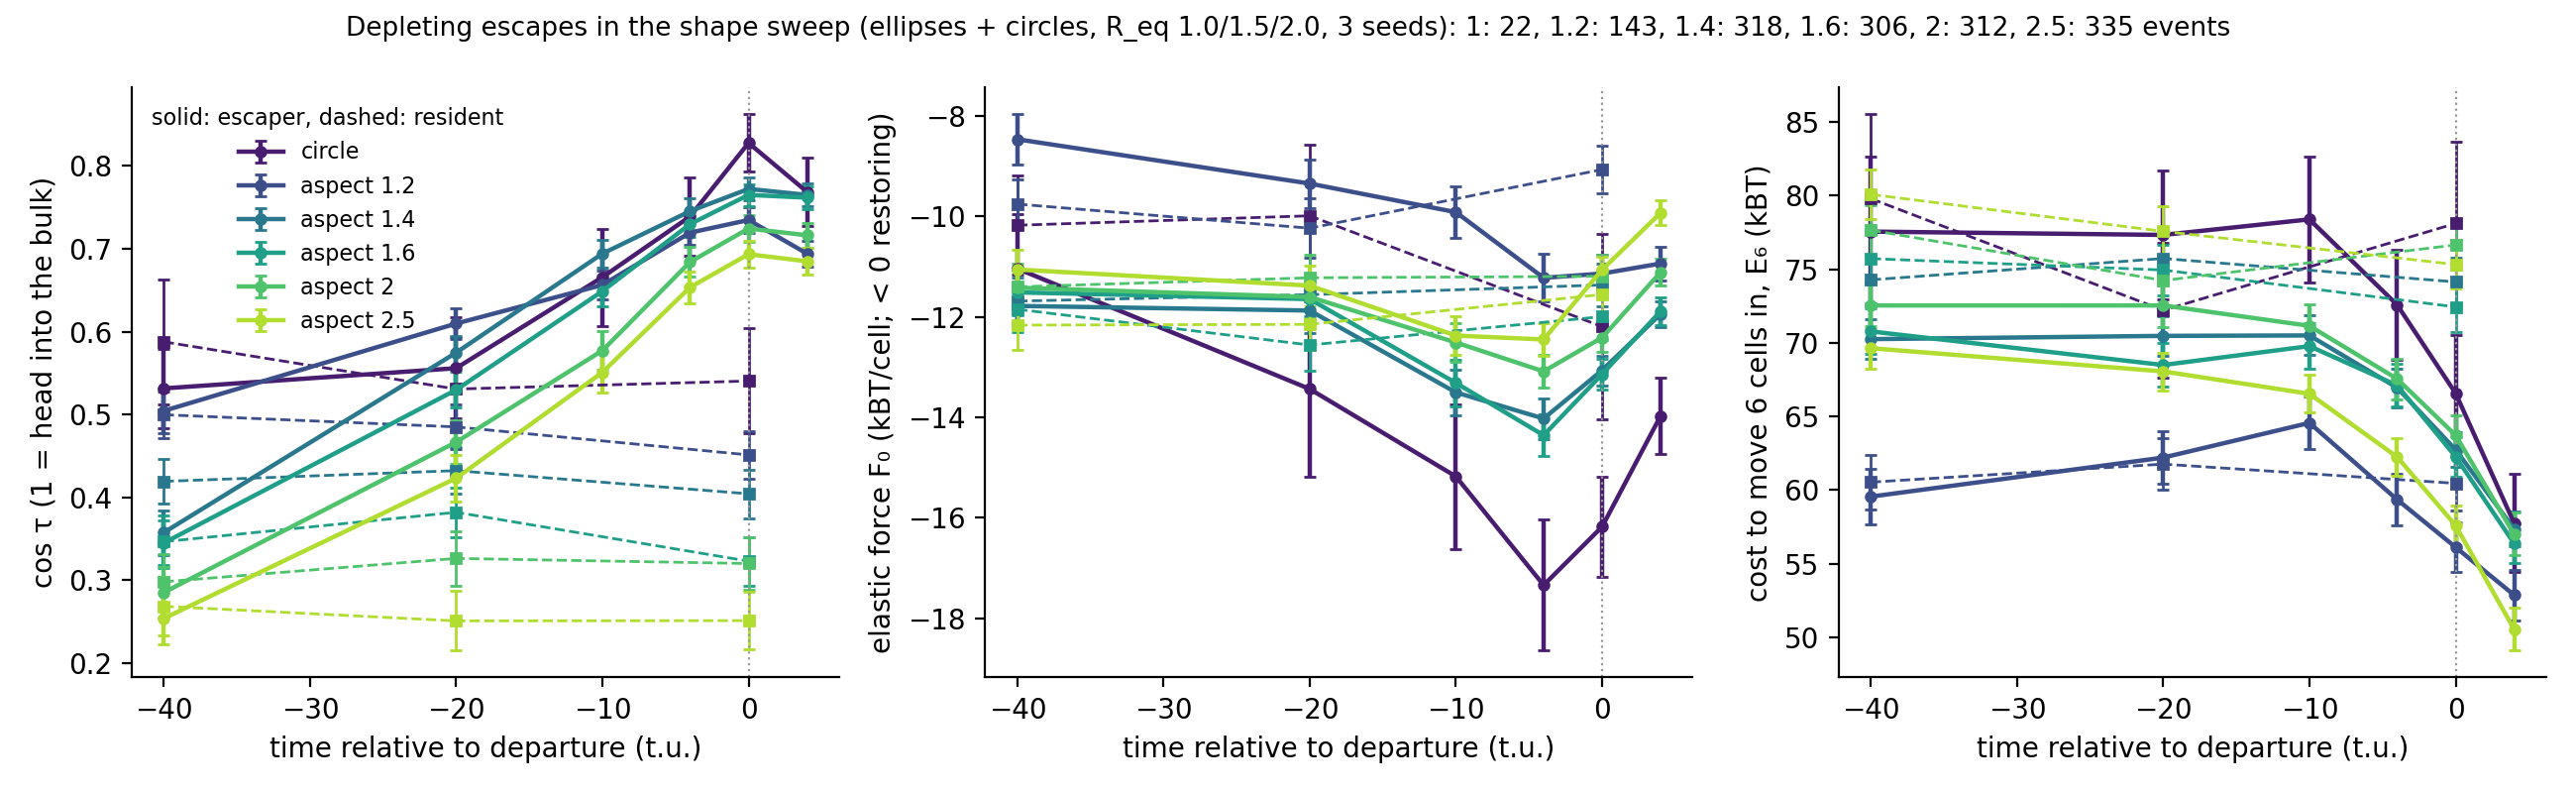
\includegraphics[width=\textwidth]{fig_etsg_shapes.png}
\caption{Depleting escapes in the shape sweep, aligned on departure, by aspect ratio (solid: escaper; dashed: random resident in the same region and frame). (a) Tilt projection
$\cos\tau$ (1 = head into the bulk); (b) elastic force $F_0$ on the defect along the inward normal ($<0$ pulls towards the wall); (c) Frank-energy cost of moving the defect 6 cells in.}\label{fig:etsg}
\end{figure}

\paragraph{Untilting first, then a local inward jet (Fig.~\ref{fig:selfflow}).}
\begin{itemize}
  \item The escaper untilts over $\approx40$\,t.u.: $\cos\tau$ rises from 0.14 at $-40$\,t.u. to 0.72 at departure, while residents stay flat. The onset is the same at every aspect and size (Fig.~\ref{fig:etsg}a).
  \item The inward flow at the defect (within 2 cells) rises only from $\approx-20$\,t.u., to 0.24 cells/t.u.\ at departure. In a ring 4--8 cells around it the flow stays flat or slightly
        \emph{outward} ($-0.01$ to $-0.02$). The burst is local to the defect.
  \item The excess flow at the core over the ring is the defect's own active jet. For free bulk $+\half$ this excess, projected on the head, is $u_\mathrm{jet}=0.32$\,cells/t.u.
        For the escaper, $u_\mathrm{jet}\cos\tau$ predicts the measured excess at departure (0.23 vs 0.24); near the wall the measured excess is $\approx0.05$ lower (see below).
  \item The defect's own inward velocity follows the flow at its core (0.08 at $-10$\,t.u., 0.34 at departure).
\end{itemize}
Untilting and the inward flow are one mechanism: the untilting turns the defect's own jet into the bulk, and the jet carries it out.

\begin{figure}[H]\centering
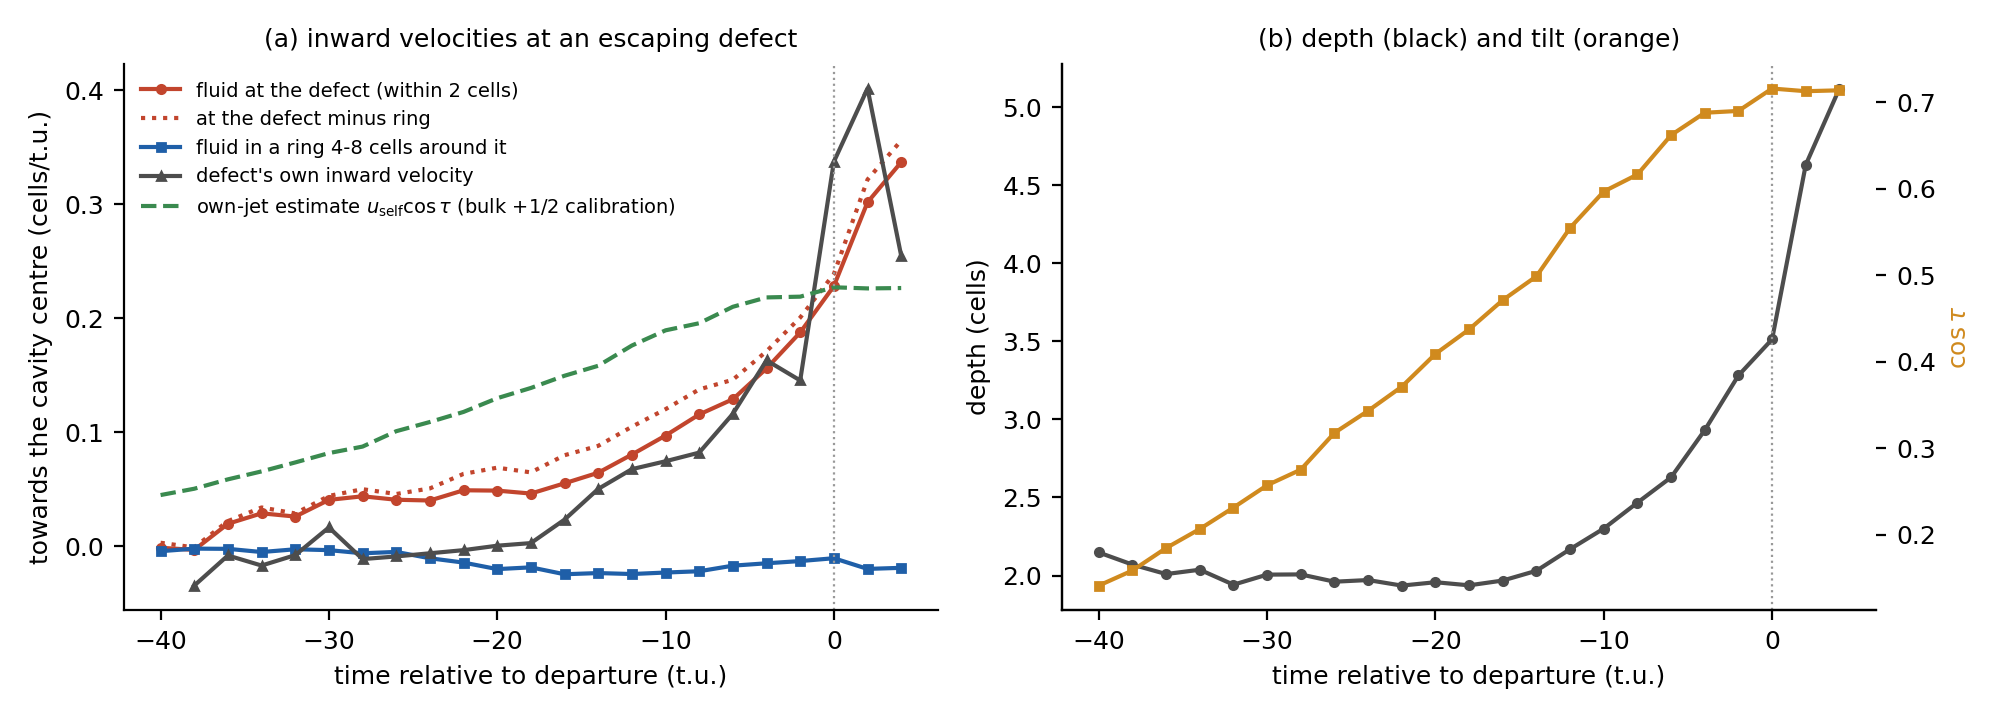
\includegraphics[width=\textwidth]{fig_selfflow_ff12.png}
\caption{Depleting escapes in the 12 fine-flow runs. (a) Inward flow (towards the cavity centre, away from the wall) at the escaper (within 2 cells), in the 4--8 cell ring, their
difference, the escaper's own inward velocity, and the own-jet estimate $u_\mathrm{jet}\cos\tau$ calibrated on free bulk $+\half$. (b) Depth and $\cos\tau$.}\label{fig:selfflow}
\end{figure}

\paragraph{The wall blocks the inward part of the jet (Fig.~\ref{fig:jetmap}).} Measured for all $+\half$ (38\,565 samples) by depth and tilt:
\begin{itemize}
  \item The jet strength along the head is \emph{not} reduced near the wall: 0.36--0.40\,cells/t.u.\ at depth 0--3 against 0.32 in the bulk.
  \item Its component along the wall normal is. The fraction transmitted, $g(d)$ (inward jet over $u_\mathrm{jet}\cos\tau$), is 0.30--0.33 within 2 cells of the wall, 0.58 at 2--3,
        0.86 at 3--4 and $\approx1$ beyond 4 cells. This is the no-penetration condition: near the wall the jet is turned along it.
  \item Closed law: inward jet $=0.40\,\cos\tau\,g(d)$. It predicts the residents' inward jet exactly (0.056 vs 0.055 at depth 2.1, $\cos\tau=0.34$).
\end{itemize}

\begin{figure}[H]\centering
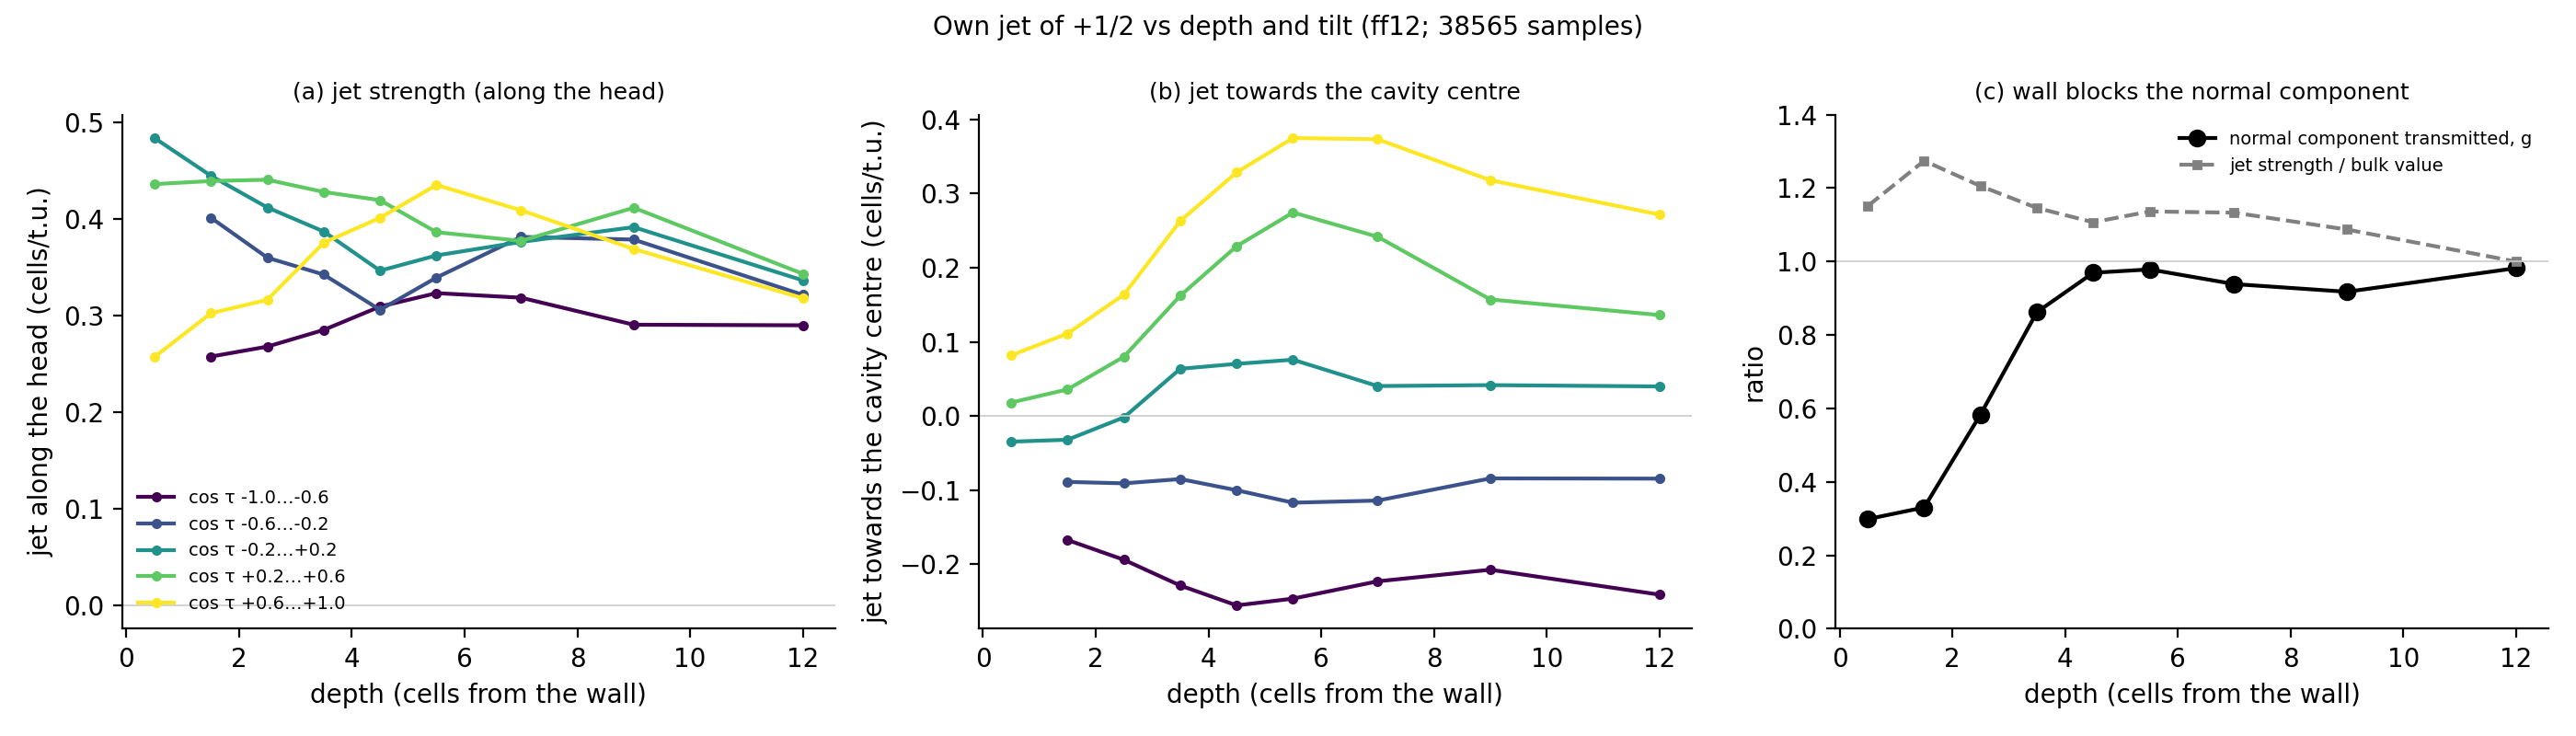
\includegraphics[width=\textwidth]{fig_jetmap_ff12.png}
\caption{Own jet of $+\half$ defects (flow within 2 cells minus the 4--8 cell ring) against depth, by tilt. (a) Strength along the head; (b) inward component; (c) transmitted fraction
of the normal component $g(d)$ and the strength relative to the bulk.}\label{fig:jetmap}
\end{figure}

\paragraph{In the flow field: the wall erases one vortex lobe (Fig.~\ref{fig:vort}).} A free $+\half$ carries two counter-rotating vortex lobes on either side of its head;
its jet is the flow between them. Measured relative to a free bulk $+\half$ (lobe vorticity 0.12/t.u.):
\begin{itemize}
  \item Near the wall the lobe on the wall side is absent: $-0.13$ of the free value at depth 1--2, 0.10 at 2--3, 0.35 at 3--4, 0.48 at 4--5, 0.60 at 5--6 and 0.78--0.86 deeper. This is the same depth scale as $g(d)$.
  \item With one lobe missing, a wall defect sits in net counter-rotating vorticity ($-0.051$/t.u.\ at depth 1--2, against $+0.02$ for bulk $+\half$).
  \item In escapers the wall-side lobe recovers \emph{before} the defect moves: 0.03, 0.08, 0.19, 0.34 and 0.46 at $-40$, $-20$, $-10$, $-4$ and 0\,t.u., and 0.7 just after departure (residents 0.07--0.14).
        At $-10$\,t.u.\ the escaper is still 2.2 cells deep, where the typical wall-side lobe is 0.10. The core vorticity of the escaper falls from $-0.033$ to $-0.003$/t.u.\ by departure (residents stay at $-0.03$): the escaper ends up riding its own symmetric flow.
\end{itemize}
Untilting swings the lobes so that the wall-side lobe leaves the wall and recovers; the dipole becomes symmetric again and the jet straightens inward.

\paragraph{Viscometric lines (Head et al., Nat.~Phys.~2024) (Fig.~\ref{fig:qcrit}).} With $\mathcal Q=\det\nabla\mathbf u$ ($=\half(\|\Omega\|^2-\|E\|^2)$ for incompressible flow; flow
smoothed over 2.5 cells, below which MPCD noise fills the cavity with $\mathcal Q=0$ lines):
\begin{itemize}
  \item MPCD reproduces their constraint. Bulk $+\half$ sit closer to $\mathcal Q=0$ lines than random points (median distance 0.85 vs 1.38 cells; large distances several times rarer).
        Bulk $-\half$ sit in rotation-dominated regions ($\mathcal Q_n=+0.26$, median distance 2.2 cells), away from the lines. Wall $+\half$ also prefer the lines (48--72\% within 1 cell vs 30--40\% for random points).
  \item Escapers land on a $\mathcal Q=0$ line as they leave: about 60\% within 1 cell until $-10$\,t.u.\ (residents 61--66\%), 89\% at departure and 91\% at $+4$\,t.u.
        Before that they pass through a rotation-dominated phase ($\mathcal Q_n=+0.10$ and $+0.13\pm0.02$ at $-20$ and $-10$\,t.u., residents $-0.06$ and 0.00), the one-sided lobe seen above.
\end{itemize}
In Head et al.'s language, an escape is the wall $+\half$ regaining the viscometric constraint of a free $+\half$. (The time course of $\mathcal Q_n$ depends on the smoothing scale;
the landing on $\mathcal Q=0$ at departure does not.)

\begin{figure}[H]\centering
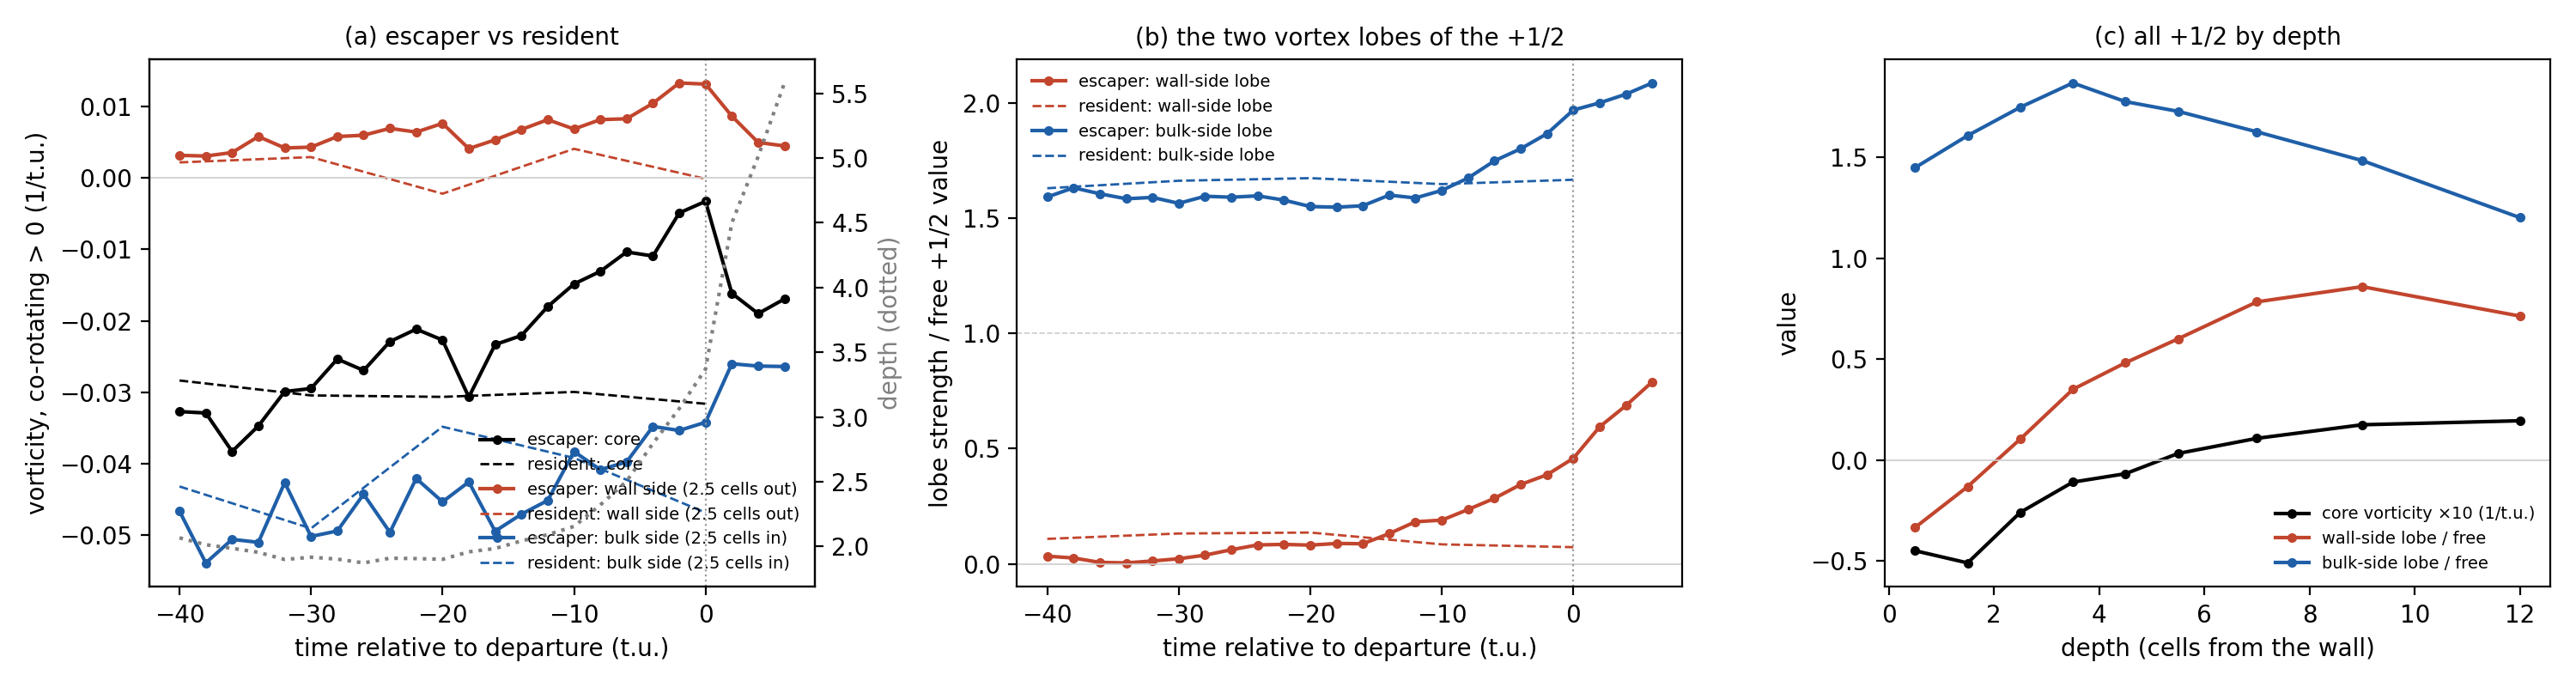
\includegraphics[width=\textwidth]{fig_vortdef_ff36.png}
\caption{Vorticity around $+\half$ defects, signed by the cavity circulation. (a) Escaper vs resident: core, 2.5 cells towards the wall and towards the bulk. (b) Strength of the escaper's
wall-side and bulk-side vortex lobes relative to a free $+\half$. (c) All $+\half$ by depth.}\label{fig:vort}
\end{figure}

\begin{figure}[H]\centering
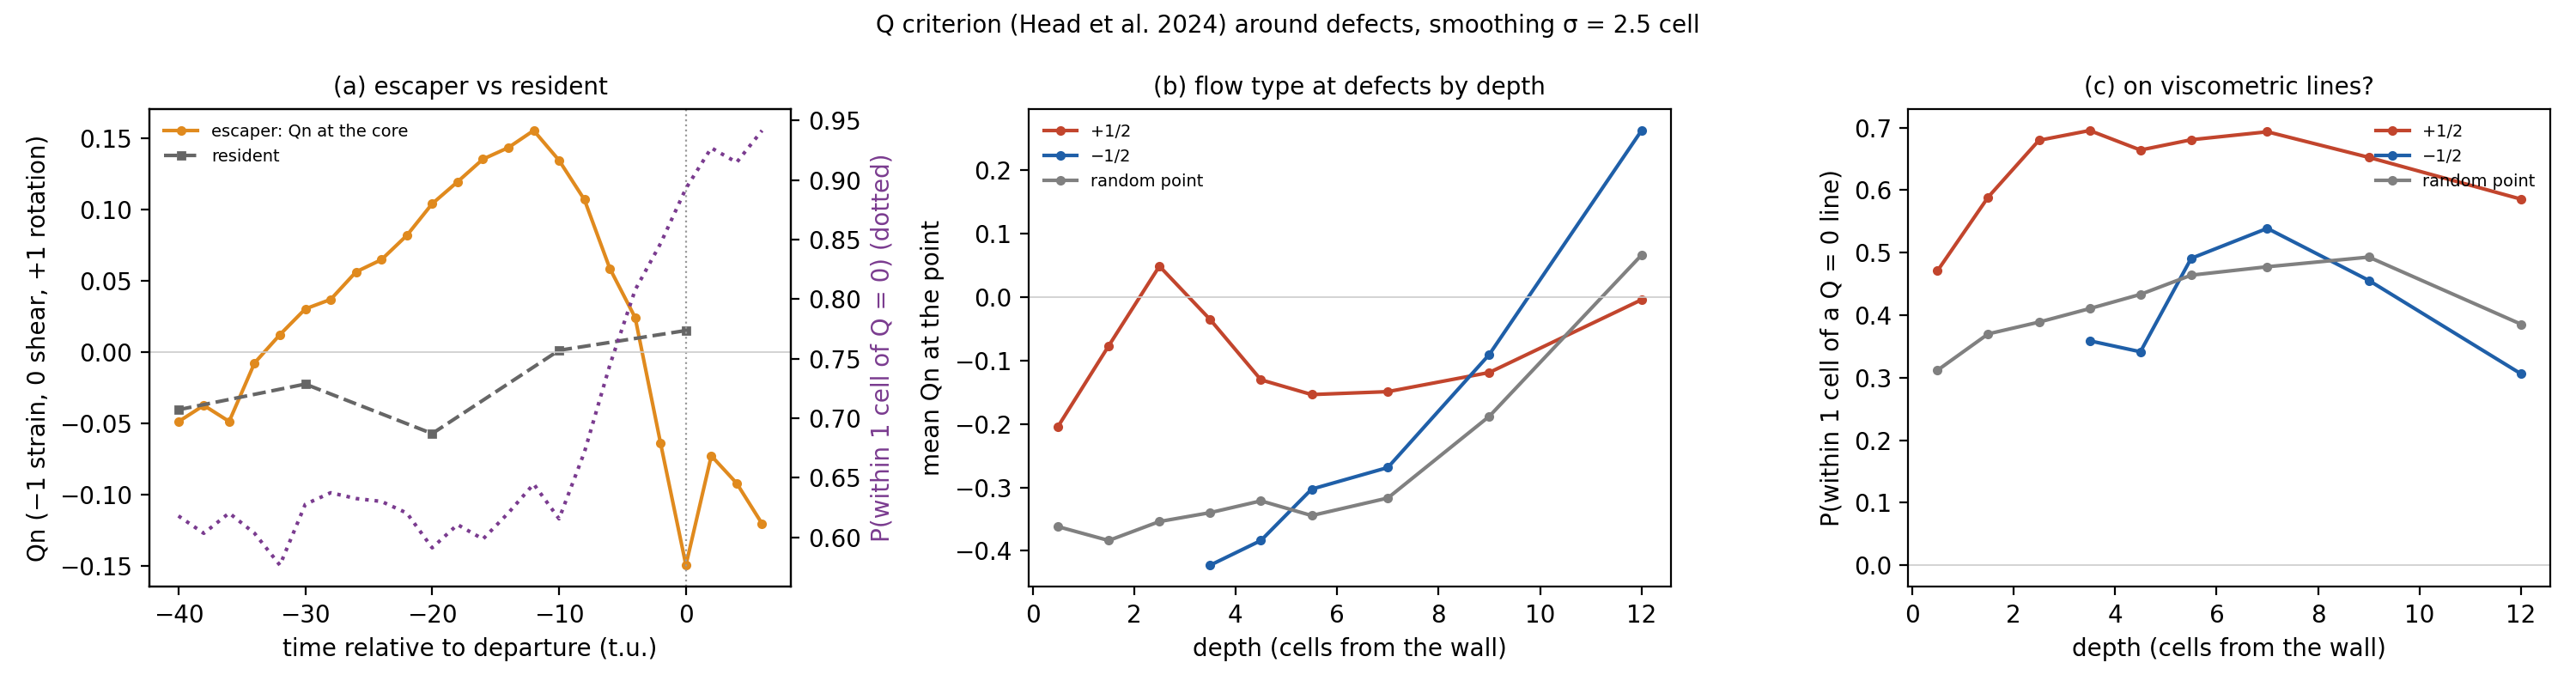
\includegraphics[width=\textwidth]{fig_qcrit_ff36s25.png}
\caption{$\mathcal Q$ criterion around defects (flow smoothed over 2.5 cells). (a) Escaper vs resident: normalised $\mathcal Q_n=(\|\Omega\|^2-\|E\|^2)/(\|\Omega\|^2+\|E\|^2)$ at the core
and the fraction within one cell of a $\mathcal Q=0$ line. (b) $\mathcal Q_n$ at $\pm\half$ and random points by depth. (c) Fraction within one cell of a $\mathcal Q=0$ line.}\label{fig:qcrit}
\end{figure}

\paragraph{Force balance.} Per frame, we fitted the escaper's inward velocity as $v_\mathrm{in}=\alpha\,u_\mathrm{jet,in}+\beta\,u_\mathrm{ring}+\mu_n F_0+c$
(own jet, background flow and elastic force, all along the inward normal; bootstrap over events):
\begin{itemize}
  \item Free bulk $+\half$: $\alpha=0.64\pm0.01$, $\beta=0.58\pm0.01$. Escapers (36 runs): $\alpha=0.87\pm0.02$, $\beta=0.98\pm0.05$, and a normal mobility $\mu_n=0.0016\pm0.0004$\,cells$^2$/($\kT$\,t.u.).
        That is about 3$\times$ below the free-defect mobility (0.0054) and more than 10$\times$ below the along-wall mobility from layer fluctuations (0.02--0.03). Treat $\mu_n$ as a lower estimate:
        $F_0$ varies little and is noisy, which biases it down.
  \item The elastic pull is therefore a drift of only $\mu_nF_0\approx-0.02$\,cells/t.u.
  \item Budget of the run-up, measured inward velocity vs model (jet, ring, elastic):
\end{itemize}
\begin{table}[H]\centering\small
\begin{tabular}{@{}rccccc@{}}\toprule
lag (t.u.) & measured $v_\mathrm{in}$ & model & jet & background & elastic \\ \midrule
$-20$ & 0.01 & 0.03 & 0.06 & $-0.03$ & $-0.02$ \\
$-10$ & 0.06 & 0.06 & 0.09 & $-0.02$ & $-0.02$ \\
$-4$  & 0.14 & 0.12 & 0.14 & $-0.01$ & $-0.02$ \\
0     & 0.36 & 0.18 & 0.19 & 0.00 & $-0.02$ \\
$+6$  & 0.31 & 0.31 & 0.33 & $-0.02$ & $-0.02$ \\ \bottomrule
\end{tabular}
\end{table}
\noindent The model tracks the run-up and misses the burst at departure, probably position jumps in the defect detection at the band edge. With the closed jet law instead of the measured jet
(tilt and depth only) the fit is somewhat worse ($R^2$ 0.21 vs 0.30) with the same $\mu_n$, and it predicts the residents' inward jet exactly (0.044 vs 0.044).

\keybox{\textbf{Escape in one paragraph.} A wall $+\half$ is held mainly by its tilt and by the wall, not by elasticity. Its jet is full strength, but the tilt points it along the wall and the
no-slip wall erases its wall-side vortex lobe, so only $\approx30\%$ of the inward component acts (about $+0.05$\,cells/t.u.). That is balanced by an elastic drift of
$\approx-0.02$ and by pinning. Untilting raises the inward projection and lets the missing lobe recover; each cell of depth then lets more of the jet act (0.33, 0.58, 0.86, 1), so the push
triples between 2 and 4 cells and the defect runs away. It leaves on a $\mathcal Q=0$ line, like a free $+\half$.}

\paragraph{Tips and flanks (Fig.~\ref{fig:etsgreg}).} Per resident wall defect, the tips leak 2--2.5$\times$ faster than the flanks at aspect $\ge1.4$. At the onset (aspect 1.2) escapes are almost only at the tips (61 vs 5 on the flanks).
From aspect 1.4 on every region leaks, and only $\approx40\%$ of escapes are at the tips. All regions share the untilting run-up, but the weak spot differs:
\begin{itemize}
  \item At the tips the whole layer is less tilted (residents $\cos\tau=0.46$ vs 0.25--0.29 elsewhere), so every tip defect already has more of its jet pointing inward. There is no elastic difference
        (escape cost 73.5 vs 75.9\,$\kT$).
  \item On the flanks and mid sections, escapes start from elastically cheaper sites: 7--9\,$\kT$ below residents from 40\,t.u.\ before, probably a gap in the layer next to the site.
  \item In the flow (36 runs: 190 tip, 140 mid, 81 flank escapes) the mechanism is the same everywhere: jet coefficient 0.82--0.90, the wall-side lobe recovers in the same way, and 87--91\% land on a $\mathcal Q=0$ line.
        At the tips the elastic pull is dynamically absent ($\mu_n=0.0005\pm0.0005$ vs 0.0024--0.0027 elsewhere) and the background flow is carried fully.
\end{itemize}

\begin{figure}[H]\centering
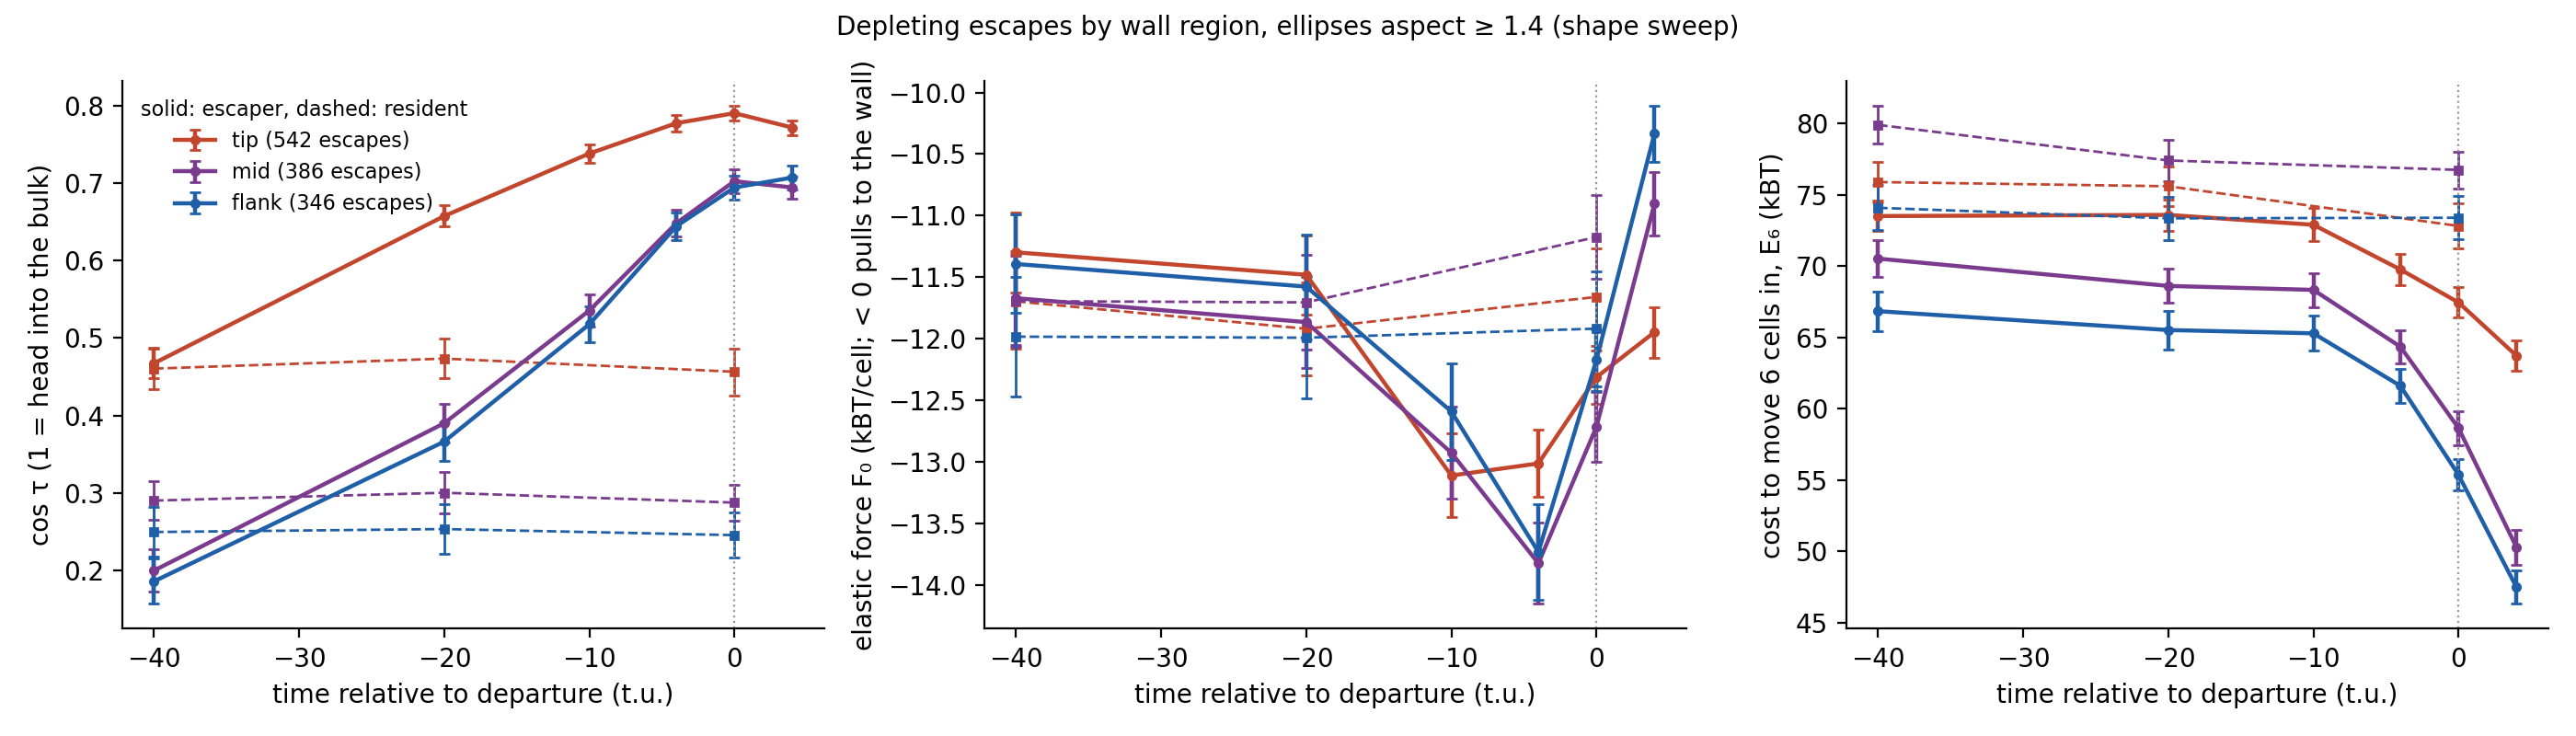
\includegraphics[width=\textwidth]{fig_etsg_reg.png}
\caption{As Fig.~\ref{fig:etsg}, by wall region (tip, mid, flank by the ellipse angle parameter), pooled over aspect $\ge1.4$.}\label{fig:etsgreg}
\end{figure}

\paragraph{Ovals.} The same analyses on the Cassini ovals of the shape sweep (405 runs) and on 12 oval runs with fine flow output (aspect 1.5 and 1.9) give the same
picture: the same untilting precursor at every aspect, the same tip weakness through a less tilted tip layer, the same crowding feedback, the own jet matching $u_\mathrm{jet}\cos\tau$ at
departure, the same lobe erasure and recovery (wall-side lobe 0.08, 0.20, 0.55 at $-20$, $-10$ and 0\,t.u.), and the same landing on $\mathcal Q=0$ lines (92\% at departure). With the elastic model rebuilt for Cassini walls, a depleted oval layer is equally far above its elastic optimum: refilling the largest gap lowers the Frank energy by 81--89\,$\kT$ at aspect 1.4--1.9. Two small
differences: within 2 cells of the wall slightly more of the jet gets through ($g\approx0.45$ vs 0.3), and the mid section of an oval leaks about as much as its tips.

\paragraph{A second route: active bulk, passive wall (Fig.~\ref{fig:bulkonly}).} With activity switched off within 4 cells of the wall (10 runs, same fine output), the layer still empties,
even in circles (0.2--1.0 depleting escapes per wall defect per 1000\,t.u.; the active circle has none). The escape kinematics look the same, but what accompanies them does not:
\begin{itemize}
  \item The wall band is quiet and strain-dominated: wall circulation 0.016--0.03 (active 0.13), $\mathcal Q_n=-0.5$ to $-0.65$ (active $\approx0$).
        A $+\half$ in the passive band keeps 20--28\% of its jet and almost no lobes.
  \item There is no untilting precursor ($\cos\tau\approx0.2$ until $-20$\,t.u.; it turns only during the motion), no own jet in the band, and the background flow is slightly \emph{inward}.
  \item The force fit leaves an unexplained inward drift ($c=+0.05\pm0.014$), possibly noise plus the selection of events.
\end{itemize}
So without wall activity there is no protection and no jet: defects drift out of a quiet wall with the background flow and fluctuations against the weak elastic hold. This route
exists only when the coherent active wall circulation is absent. It is how bulk-only activity empties the layer even in circles.

\begin{figure}[H]\centering
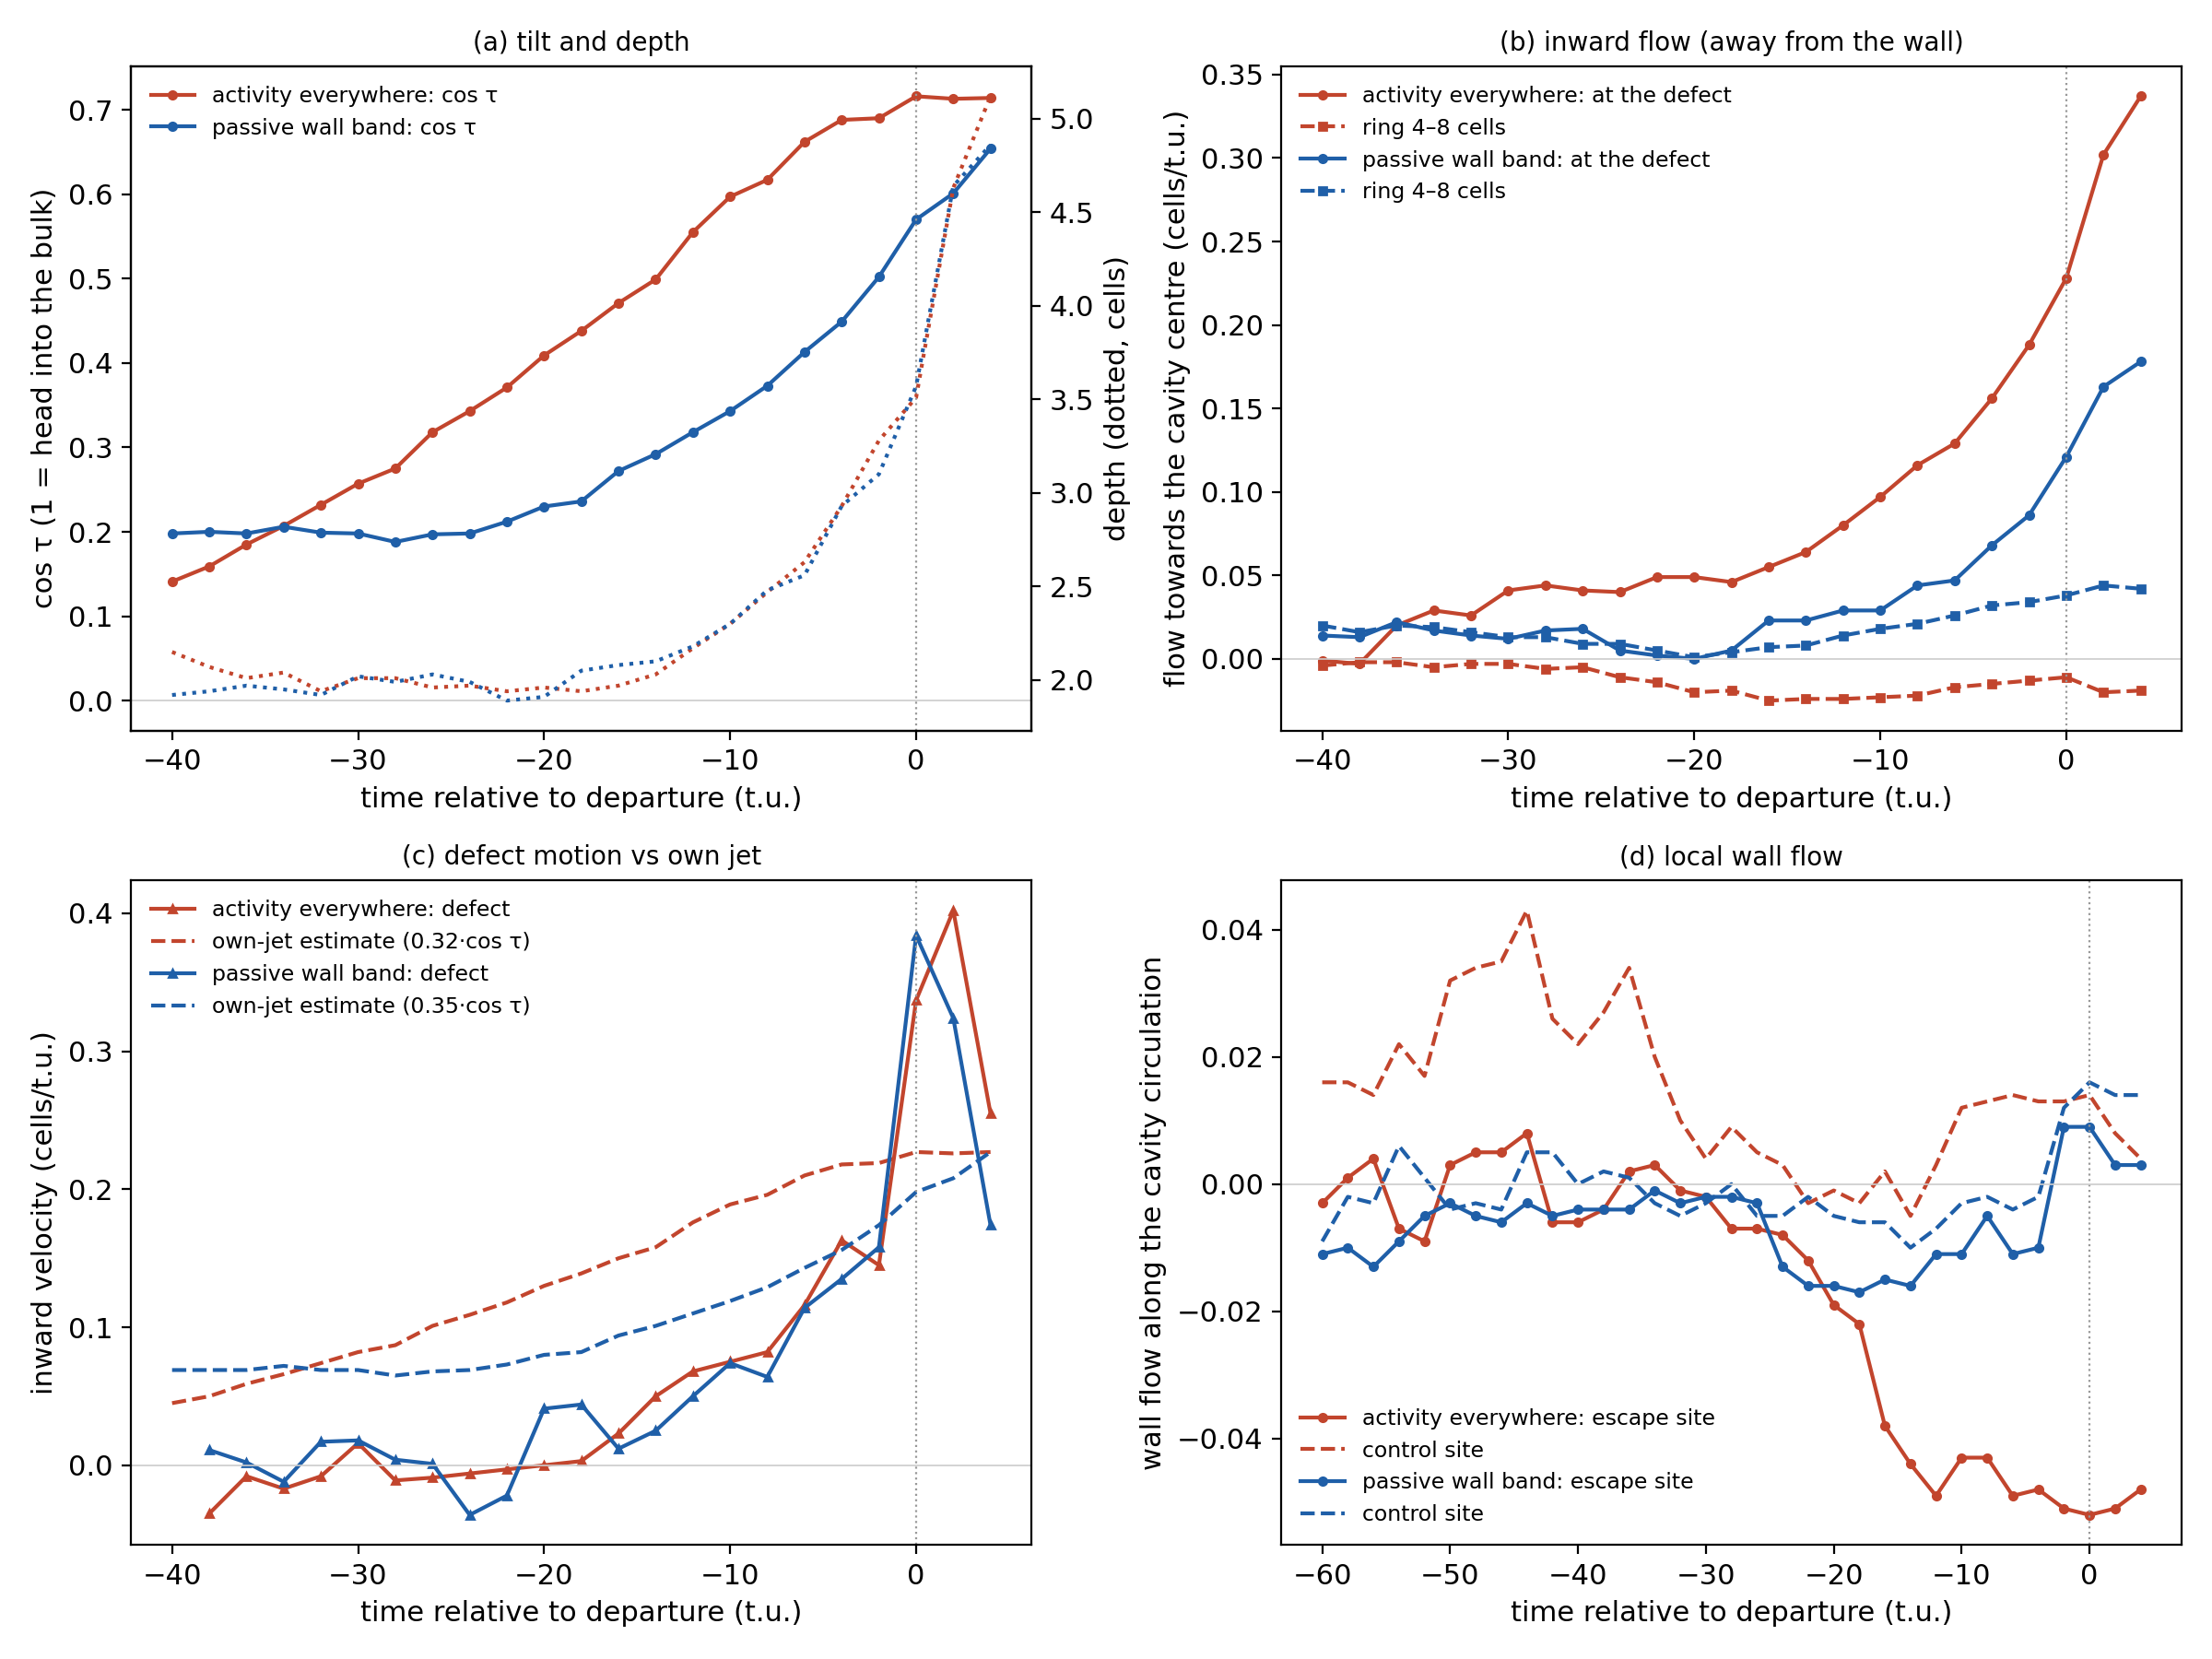
\includegraphics[width=0.85\textwidth]{fig_compare_bulk.png}
\caption{Depleting escapes with activity everywhere (red) vs activity only beyond 4 cells from the wall (blue). (a) Tilt and depth; (b) inward flow at the defect and in the 4--8 cell
ring; (c) the defect's inward velocity and the own-jet estimate; (d) local flow along the wall, signed by the cavity circulation, at the escape site and at a control site.}\label{fig:bulkonly}
\end{figure}

\paragraph{Rates are not the steady state: the $\lambda$ test.} Changing the flow-alignment parameter changes the tilt, and with it the escape rate, as the mechanism predicts. In the
aspect-2 ellipse, going from $\lambda=1.2$ to 2 to 4, the residents' $\cos\tau$ falls (0.24, 0.19, 0.14) and the depleting-escape rate falls 15$\times$ (1.01, 0.65, 0.066 per wall
defect per 1000\,t.u.). The flow gets \emph{stronger} with $\lambda$ ($v_\mathrm{rms}$ 0.46, 0.57, 0.70), so this is not a weaker-flow effect. But entries slow too: from $\lambda=2$ to 4
exits drop 6$\times$ and refills of a vacancy 3.7$\times$. The wall count barely moves (7.1, 7.1, 7.65 instead of 10). The tilt and the jet blocking set how fast defects cross the wall band
in both directions; they do not set how many the wall keeps. At $\lambda=1.2$ even the circle loses the overcharged state (wall 7.9, bulk $+2.05$, wall circulation a third of $\lambda=2$).

\paragraph{What sets the steady state? A dynamical balance far from the elastic optimum.}
\begin{itemize}
  \item \textbf{The depleted layer is not an elastic minimum.} In measured steady-state configurations, moving one bulk $+\half$ into the largest wall gap \emph{lowers} the Frank
        energy by 80--100\,$\kT$ in elongated cavities (median of the best mover; favourable in 75--100\% of frames), while ejecting a wall $+\half$ costs 50--85\,$\kT$.
        Even in the circle an extra wall defect is favourable ($-28\,\kT$), as expected since passive cavities keep all $2k$ at the wall. The overcharged bulk ($+1$ in circles,
        $+2.2$ to $+2.5$ in elongated cavities) is held up by the active dynamics against a large elastic preference for a full wall. (The passive point-defect model ignores the active tilt.)
  \item \textbf{The bulk charge limits itself through the exits} (B.~Loewe's hypothesis). Within runs (49 elongated runs, $\approx195\,000$ wall-defect frames), when the bulk charge is
        above its run average the wall defects exit less often: relative to the average, 1.9$\times$ at one unit below and 0.9$\times$ at one unit above.
        \begin{itemize}
          \item Not through the jet: the wall defects sit closer to the wall (0.12 cell per unit of charge), but they are also less tilted, so their inward jet push is unchanged.
          \item Not through bulk pressure: the push of the bulk charges on wall defects (2D defect interaction) is the same at tips, mid and flanks at every aspect, and adding it to the
                per-defect model explains little.
          \item \emph{Through the crowding of the layer.} The exit rate per wall defect falls as the layer empties: 0.068 per 20\,t.u.\ for a full layer of $2k-2$, 0.050, 0.037 and 0.028 with one,
                two and five vacancies. With crowding included the per-defect model reproduces most of the trend. A sparser layer holds its remaining defects more strongly; in the
                elastic model a vacancy makes its neighbours more bound by 8--10\,$\kT$. As the bulk charges up, the wall empties and each remaining wall defect sits in a deeper well.
        \end{itemize}
  \item \textbf{Refill.} Entries per vacancy fall with the bulk charge, but the total entry flux rises (0.11$\to$0.39 per frame), because vacancies grow faster. Both fluxes are restoring.
        Refill is slowed by the same tilt and jet blocking as the exits (the $\lambda$ test).
  \item \textbf{The steady state is unique.} Runs seeded with 10, 7 or 4 wall defects (aspect 2, $k=6$, 4 seeds each, seeding through a new initial-director option) all converge to
        $7.2\pm0.1$ wall defects and bulk $+2.4$ within 300--700\,t.u., the value of unseeded runs. Circles seeded with 12 (the passive arrangement) or 6 wall defects both end at $2k-2=10$ with bulk $+1.0$.
\end{itemize}
The steady state sits where an exit flux that falls as the layer empties meets a refill flux that rises with the vacancies, far above the elastic optimum. The tilt sets how fast both
fluxes run; the geometry (through the coherence of the flow) sets where they cross.
% TODO after runs/lambda_circle: tilt law across lambda in active circles, and the lambda range where the circle state survives (lambda 1.2 already loses it).
